\documentclass[table]{beamer}

\usepackage[spanish]{babel}
\usepackage[normalem]{ulem}
\usepackage{xcolor}
\usepackage{pgfgantt}
\usepackage{booktabs}
\usepackage{bookmark}
\usepackage{tabularx}
\usepackage{graphicx}
\usepackage{pgfplots}
\pgfplotsset{compat=newest}

\usepackage{tikz}
\usetikzlibrary{shapes.geometric, arrows.meta, fit, backgrounds, positioning, matrix, decorations.pathreplacing, calc}
\tikzstyle{startstop} = [rectangle, rounded corners, minimum width=3cm, minimum height=1cm,text centered, draw=black, fill=red!50]
\tikzstyle{io} = [trapezium, trapezium left angle=70, trapezium right angle=110, minimum width=3cm, minimum height=1cm, text centered, draw=black, fill=blue!30]
\tikzstyle{process} = [rectangle, minimum width=3cm, minimum height=1cm, text centered, draw=black, fill=orange!30]
\tikzstyle{decision} = [diamond, minimum width=3cm, minimum height=1cm, text centered, draw=black, fill=green!20]
\tikzstyle{database} = [cylinder, minimum width=3cm, minimum height=2cm, text centered, shape border rotate=90, aspect=0.25, draw=black, fill=yellow!30]
\tikzstyle{arrow} = [thick, ->, >=stealth]
\tikzstyle{line} = [-Latex]

\newcommand{\inline}[2]{%
    \begin{tikzpicture}[baseline=(word.base), txt/.style={shape=rectangle, inner sep=0pt}]
        \node[txt] (word) {\texttt{#1}};
        \node[above] at (word.north) {\footnotesize{#2}};
    \end{tikzpicture}%
}

\newlength\figureheight
\newlength\figurewidth
\setlength\figureheight{0.7\linewidth}
\setlength\figurewidth{\linewidth}

\usetheme{metropolis}

\title{Estudio sobre Sistemas de Recomendación y Predicción basados en el procesamiento del lenguaje natural}
\date{\today}
\author{Hugo Ferrando Seage}
\institute{Universidad Europea de Madrid\\Escuela de Arquitectura, Ingeniería y Diseño}

\begin{document}
  \maketitle

  \section{Introducción}
  \begin{frame}{Introducción}
      Los recomendadores son una parte esencial de cualquier servicio de Video on Demand (VOD). Tanto Netflix como Movistar+, Amazon, Hulu y HBO cuentan con sus propios sistemas.

      También existen webs que usan sus recomendadores, como IMDb o FilmAffinity. Incluso existen servicios comerciales que se dedican a productivizar su sistema de recomendación, como Jinni.
  \end{frame}

  \begin{frame}{Introducción}
      Existen tres grandes tipos de sistemas de recomendación:
      \begin{itemize}
          \item Filtrado Colaborativo
          \item Filtrado por contenido
          \item Sistemas híbridos
      \end{itemize}
  \end{frame}

  \begin{frame}{Filtrado Colaborativo}
      Consiste en emparejar usuarios que tengan gustos similares y recomendar en base a esos datos.

      Normalmente se representa usando una matriz bidimensional donde las filas representan usuarios y la columnas representan productos.

      Los usuarios deben puntuar los contenidos, o se pueden usar otras métricas.
  \end{frame}

  \begin{frame}{Filtrado por Contenido}
      Consiste en la creación de un modelo que determina la similitud entre productos en base a algún criterio.

      Ese criterio puede ser cualquier elemento del producto. Para películas puede ser el género. Para restaurantes el tipo de cocina. Etc.
  \end{frame}

  \begin{frame}{Filtrado Híbrido}
      Usan una combinación de ambas técnicas para complementar las recomendaciones.
  \end{frame}

  \section{Objetivos}

  \begin{frame}{Objetivos}
      \begin{itemize}
          \item Construir un recomendador de películas
          \item Crear el modelo en base a tres algoritmos
              \begin{itemize}
                  \item LSA
                  \item Doc2Vec
                  \item E-Modelo
              \end{itemize}
          \item Optimizar modelos
          \item Crear una interfaz desde donde poder probarlos
      \end{itemize}
  \end{frame}

  \section{Metodología}

  \begin{frame}{Metodología}
      La metodología usada ha sido ágil, basada en MVPs.

      \begin{figure}[!htbp]
          \resizebox{0.45\textwidth}{!}{
              \centering
              \begin{ganttchart}[
                  hgrid,
                  vgrid,
                  time slot format=isodate-yearmonth,
                  compress calendar
                  ]{2016-9}{2017-7}
                  \setganttlinklabel{f-s}{}

                  \gantttitlecalendar{year, month} \\
                  \ganttbar{Investigación}{2016-09}{2016-11} \\
                  \ganttbar{Doc2Vec}{2017-03}{2017-03} \\
                  \ganttbar{LSA MVP1}{2016-10}{2016-11} \\
                  \ganttbar{LSA MVP2}{2016-12}{2017-01} \\
                  \ganttbar{LSA MVP3}{2017-02}{2017-03} \\
                  \ganttbar{ALS MVP1}{2016-09}{2016-12} \\
                  \ganttbar{ALS MVP2}{2017-01}{2017-02} \\
                  \ganttbar{ALS MVP3}{2017-03}{2017-03} \\
                  \ganttbar{Desarrollo Interfaz}{2017-04}{2017-05} \\
                  \ganttmilestone{Fin Desarrollo}{2017-05} \\
                  \ganttbar{Documentación}{2017-05}{2017-06} \\
                  \ganttmilestone{Entrega \& Presentación}{2017-06}{2017-06}

                  \ganttlink{elem0}{elem1}
                  \ganttlink{elem0}{elem2}

                  \ganttlink[link type=f-s]{elem2}{elem3}
                  \ganttlink[link type=f-s]{elem3}{elem4}

                  \ganttlink[link type=f-s]{elem5}{elem6}
                  \ganttlink[link type=f-s]{elem6}{elem7}

                  \ganttlink[link type=f-s]{elem1}{elem8}
                  \ganttlink[link type=f-s]{elem4}{elem8}
                  \ganttlink[link type=f-s]{elem7}{elem8}

                  \ganttlink{elem8}{elem9}
                  \ganttlink{elem10}{elem11}
              \end{ganttchart}
          }
      \end{figure}
  \end{frame}

  \section{Descarga de datos}

  \begin{frame}{Descarga de datos}
      Para entrenar los modelos es necesario obtener una gran cantidad de textos. Para ello se ha creado un crawler usando Spidy, que descarga información y críticas de las top 1000 películas de IMDb.
  \end{frame}

  \begin{frame}{Descarga de datos}
      \begin{figure}[!htbp]
          \resizebox{0.45\textwidth}{!}{
              \begin{tikzpicture}[node distance=2cm]
                  \centering
                  \node (init) [startstop] {Top 1000 IMDb};
                  \node (link1) [decision, below of=init] {URL};
                  \node (pelicula-init) [startstop, below of=link1] {Película};
                  \node (link2) [decision, below of=pelicula-init, yshift=-2cm] {URL};
                  \node (keywords) [process, right of=link2, xshift=2cm] {Palabras clave};
                  \node (info) [process, above of=keywords] {Información};
                  \node (reviews) [startstop, below of=link2] {Críticas};
                  \node (link3) [decision, below of=reviews] {URL};
                  \node (reviews-1) [process, right of=reviews, xshift=2cm] {Crítica};
                  \node (database) [database, right of=link1, xshift=3cm] {BD};
                  \begin{scope}[on background layer]
                      \node (bbox) [rectangle,draw,minimum width=2cm] [fit = (info) (keywords) (reviews-1),fill=yellow!30,label=above:Película] {};
                  \end{scope}

                  \draw [line] (init) -- (link1);
                  \draw [line] (link1) to [bend left] node[anchor=east] {página} (init);
                  \draw [line] (link1) -- node[anchor=north] {¿visitado?} (database);
                  \draw [line] (database) |- node[anchor=west] {no} (pelicula-init);
                  \draw [line] (pelicula-init) -- (link2);
                  \draw [line] (pelicula-init) |- (info);
                  \draw [line] (link2) -- (keywords);
                  \draw [line] (link2) -- (reviews);
                  \draw [line] (reviews) -- (link3);
                  \draw [line] (link3) to [bend left] node[anchor=east] {página} (reviews);
                  \draw [line] (link3) -| (reviews-1);
              \end{tikzpicture}
          }
      \end{figure}
  \end{frame}

  \section{Limpieza de textos}

  \begin{frame}{Limpieza de textos}
      Antes de crear los modelos es necesario hacer un pretratado de los textos.
  \end{frame}

  \begin{frame}[fragile]{Ejemplo}
      \begin{verbatim}
          Zeus is a Greek God.
      \end{verbatim}
  \end{frame}

  \begin{frame}[fragile]{POS Tagger}
      \begin{figure}[!htbp]
          \centering
          \inline{Zeus}{NNP} \inline{is}{VBZ} \inline{a}{DT} \inline{Greek}{NN} \inline{God}{NNP}.
      \end{figure}
  \end{frame}

  \begin{frame}[fragile]{Hiperónimos}
      \begin{verbatim}
          Zeus is a country deity.
      \end{verbatim}
  \end{frame}

  \begin{frame}[fragile]{Nombres propios}
      Es necesario eliminar los nombres propios para que no se relacionen películas con personajes que tienen el mismo nombre.
      \begin{verbatim}
          is a country deity.
      \end{verbatim}
  \end{frame}

  \begin{frame}[fragile]{Stopwords}
      \begin{verbatim}
          country deity
      \end{verbatim}
  \end{frame}

  \begin{frame}[fragile]{Stemmer}
      \begin{verbatim}
          counti deiti
      \end{verbatim}
  \end{frame}

  \section{LSA}

  \begin{frame}{LSA}
      Latent Semantic Analysis trata de extraer conceptos de cada texto y analizar la relación entre documentos.
  \end{frame}

  \begin{frame}[fragile]{TF-IDF}
      Term Frequency-Inverse Document Frequency calcula lo relevante que es cada palabra del vocabulario dentro de cada texto.
      \tiny
      \[tfidf =
          \begin{tikzpicture}[baseline=-0.65ex,scale=0.8]
              \matrix [matrix of math nodes,left delimiter=(,right delimiter=),row sep=0.5cm,column sep=0.5cm] (m) {
                  0.39&0.16&0.19&0.01&0.25&0.79&0.27 \\
                  0.12&0.12&0.06&0.46&0.21&0.07&0.83 \\
                  0.46&0.55&0.15&0.55&0.22&0.27&0.11 \\
                  0.00&0.60&0.51&0.00&0.00&0.60&0.00 \\
                  0.41&0.00&0.35&0.83&0.00&0.00&0.00 \\
              };
              \node[above=10pt of m-1-1, rotate=45, yshift=3mm, xshift=3mm] (top-1) {says};
              \node[above=10pt of m-1-2, rotate=45, yshift=3mm, xshift=3mm] (top-2) {just};
              \node[above=10pt of m-1-3, rotate=45, yshift=3mm, xshift=3mm] (top-3) {room};
              \node[above=10pt of m-1-4, rotate=45, yshift=3mm, xshift=3mm] (top-4) {dead};
              \node[above=10pt of m-1-5, rotate=45, yshift=3mm, xshift=3mm] (top-5) {asks};
              \node[above=10pt of m-1-6, rotate=45, yshift=3mm, xshift=3mm] (top-6) {ship};
              \node[above=10pt of m-1-7, rotate=45, yshift=3mm, xshift=3mm] (top-7) {mother};

              \node[left=12pt of m-1-1] (left-1) {The Matrix};
              \node[left=12pt of m-2-1] (left-2) {Alien};
              \node[left=12pt of m-3-1] (left-3) {Serenity};
              \node[left=12pt of m-4-1] (left-4) {Casablanca};
              \node[left=12pt of m-5-1] (left-5) {Amelie};
          \end{tikzpicture}
      \]
  \end{frame}

  \begin{frame}{SVD}
      El siguiente paso es descomponer la matriz en valores singulares.
  \end{frame}

  \begin{frame}[fragile]{SVD}
      Matriz Palabra-Concepto.
      \tiny
      \[
          U =
          \begin{tikzpicture}[baseline=-0.65ex,scale=0.8]
              \matrix [matrix of math nodes,left delimiter=(,right delimiter=),row sep=0.5cm,column sep=0.5cm] (m) {
                  0.13&0.02&-0.01& \\
                  0.41&0.07&-0.03& \\
                  0.55&0.09&-0.04& \\
                  0.68&0.11&-0.05& \\
                  0.15&-0.59&0.65& \\
                  0.07&-0.73&0.67& \\
                  0.07&-0.29&0.32& \\
              };

              \node[above=10pt of m-1-1, rotate=45, yshift=3mm, xshift=5mm] (top-1) {Sci-Fi topic};
              \node[above=10pt of m-1-2, rotate=45, yshift=3mm, xshift=5mm] (top-2) {Romance topic};
              \node[above=10pt of m-1-3, rotate=45, yshift=3mm, xshift=5mm] (top-3) {Ruido};

              \node[left=12pt of m-1-1] (left-1) {action};
              \node[left=12pt of m-2-1] (left-2) {gun};
              \node[left=12pt of m-3-1] (left-3) {shoot};
              \node[left=12pt of m-4-1] (left-4) {run};
              \node[left=12pt of m-5-1] (left-5) {love};
              \node[left=12pt of m-6-1] (left-6) {peace};
              \node[left=12pt of m-7-1] (left-7) {kiss};

          \end{tikzpicture}
      \]
  \end{frame}

  \begin{frame}[fragile]{SVD}
      Matriz de relevancia de Conceptos.
      \tiny
      \[
          \Sigma =
          \begin{tikzpicture}[baseline=-0.65ex,scale=0.8]
              \matrix [matrix of math nodes,left delimiter=(,right delimiter=),row sep=0.5cm,column sep=0.5cm] (m) {
                  12.4&0&0& \\
                  0&9.5&0& \\
                  0&0&1.3& \\
              };

              \node[above=10pt of m-1-1, rotate=45, yshift=3mm, xshift=5mm] (top-1) {Sci-Fi topic};
              \node[above=10pt of m-1-2, rotate=45, yshift=3mm, xshift=5mm] (top-2) {Romance topic};
              \node[above=10pt of m-1-3, rotate=45, yshift=3mm, xshift=5mm] (top-3) {Ruido};
          \end{tikzpicture}
      \]
  \end{frame}

  \begin{frame}[fragile]{SVD}
      Matriz Película-Concepto.
      \tiny
      \[
          V^T =
          \begin{tikzpicture}[baseline=-0.65ex,scale=0.8]
              \matrix [matrix of math nodes,left delimiter=(,right delimiter=),row sep=0.5cm,column sep=0.5cm] (m) {
                  0.56&0.59&0.56&0.09&0.09 \\
                  0.12&-0.02&0.12&-0.69&-0.69 \\
                  0.40&-0.80&0.40&0.09&0.09 \\};

              \node[above=10pt of m-1-1, rotate=45, yshift=3mm, xshift=3mm] (top-1) {Matrix};
              \node[above=10pt of m-1-2, rotate=45, yshift=3mm, xshift=3mm] (top-2) {Alien};
              \node[above=10pt of m-1-3, rotate=45, yshift=3mm, xshift=3mm] (top-3) {Serenity};
              \node[above=10pt of m-1-4, rotate=45, yshift=3mm, xshift=3mm] (top-4) {Casablanca};
              \node[above=10pt of m-1-5, rotate=45, yshift=3mm, xshift=3mm] (top-5) {Amelie};

              \node[left=12pt of m-1-1] (left-1) {Sci-Fi topic};
              \node[left=12pt of m-2-1] (left-2) {Romance topic};
              \node[left=12pt of m-3-1] (left-3) {Ruido};

          \end{tikzpicture}
      \]
  \end{frame}

  \begin{frame}[fragile]{SVD}
      Los conceptos menos relevantes se pueden eliminar.
      \tiny
      \[
          V^T =
          \begin{tikzpicture}[baseline=-0.65ex,scale=0.8]
              \matrix [matrix of math nodes,left delimiter=(,right delimiter=),row sep=0.5cm,column sep=0.5cm] (m) {
                  0.56&0.59&0.56&0.09&0.09 \\
                  0.12&-0.02&0.12&-0.69&-0.69 \\};

              \node[above=10pt of m-1-1, rotate=45, yshift=3mm, xshift=3mm] (top-1) {Matrix};
              \node[above=10pt of m-1-2, rotate=45, yshift=3mm, xshift=3mm] (top-2) {Alien};
              \node[above=10pt of m-1-3, rotate=45, yshift=3mm, xshift=3mm] (top-3) {Serenity};
              \node[above=10pt of m-1-4, rotate=45, yshift=3mm, xshift=3mm] (top-4) {Casablanca};
              \node[above=10pt of m-1-5, rotate=45, yshift=3mm, xshift=3mm] (top-5) {Amelie};

              \node[left=12pt of m-1-1] (left-1) {Sci-Fi topic};
              \node[left=12pt of m-2-1] (left-2) {Romance topic};

          \end{tikzpicture}
      \]
  \end{frame}

  \begin{frame}{Similitud Coseno}
      \begin{figure}[!htbp]
          \begin{equation}
              \cos\left(
                  \begin{tikzpicture}[baseline=-0.65ex,scale=0.8]
                      \matrix [matrix of math nodes,left delimiter=(,right delimiter=),row sep=0.5cm,column sep=0.5cm] (m) {0.56\\0.12\\};
                  \end{tikzpicture}
                  ,
                  \begin{tikzpicture}[baseline=-0.65ex,scale=0.8]
                      \matrix [matrix of math nodes,left delimiter=(,right delimiter=),row sep=0.5cm,column sep=0.5cm] (m) {0.59\\-0.02\\};
                  \end{tikzpicture}
              \right) = 0.97
          \end{equation}
          \caption{Alta similitud entre Matrix y Alien}
      \end{figure}

      \begin{figure}[!htbp]
          \begin{equation}
              \cos\left(
                  \begin{tikzpicture}[baseline=-0.65ex,scale=0.8]
                      \matrix [matrix of math nodes,left delimiter=(,right delimiter=),row sep=0.5cm,column sep=0.5cm] (m) {0.56\\0.12\\};
                  \end{tikzpicture}
                  ,
                  \begin{tikzpicture}[baseline=-0.65ex,scale=0.8]
                      \matrix [matrix of math nodes,left delimiter=(,right delimiter=),row sep=0.5cm,column sep=0.5cm] (m) {0.09\\-0.69\\};
                  \end{tikzpicture}
              \right) = -0.08
          \end{equation}
          \caption{Baja similitud entre Matrix y Amelie}
      \end{figure}
  \end{frame}

  \section{Doc2Vec}

  \begin{frame}{Word2Vec}
      Word2Vec es un algoritmo creado por Google en 2013. Es conceptualmente similar a LSA, pero teniendo en cuenta cada palabra dentro de su contexto.

      Es decir, calcula la probabilidad de que una palabra esté en la vecindad de otra palabra en el vocabulario.
  \end{frame}

  \begin{frame}{Word2Vec}
      En primer lugar se guardan las parejas de palabras dentro de una ventana.
      \tiny
      \begin{table}
          \centering
          \begin{tabular}{cp{45mm}}
              \toprule
              Source Text & Training Samples \\
              \midrule
              \colorbox{blue!20}{\colorbox{red!20}{The} quick brown} fox jumps over the lazy dog & (`the', `quick') \newline (`the', `brown') \\
              \midrule
              \colorbox{blue!20}{The \colorbox{red!20}{quick} brown fox} jumps over the lazy dog & (`quick', `the') \newline (`quick', `brown') \newline (`quick', `fox') \\
              \midrule
              \colorbox{blue!20}{The quick \colorbox{red!20}{brown} fox jumps} over the lazy dog & (`brown', `the') \newline (`brown', `quick') \newline (`brown', `fox') \newline (`brown', `jumps') \\
              \midrule
              The \colorbox{blue!20}{quick brown \colorbox{red!20}{fox} jumps over} the lazy dog & (`fox', `quick') \newline (`fox', `brown') \newline (`fox', `jumps') \newline (`fox', `over') \\
              \bottomrule
          \end{tabular}
      \end{table}
  \end{frame}

  \begin{frame}{Word2Vec}
      Las palabras del vocabulario se convierten a vectores one-hot.

      \begin{table}
          \centering
          \begin{tabular}{ccc}
              \toprule
              Palabra & Posición por orden alfabético & Vector\\
              \midrule
              fox & 2/3 & [0, 1, 0]\\
              dog & 1/3 & [1, 0, 0]\\
              zebra & 3/3 & [0, 0, 1]\\
              \bottomrule
          \end{tabular}
      \end{table}
  \end{frame}

  \begin{frame}{Word2Vec}
      Con los datos obtenidos se entrena una red neuronal con una capa oculta.

      \centering
      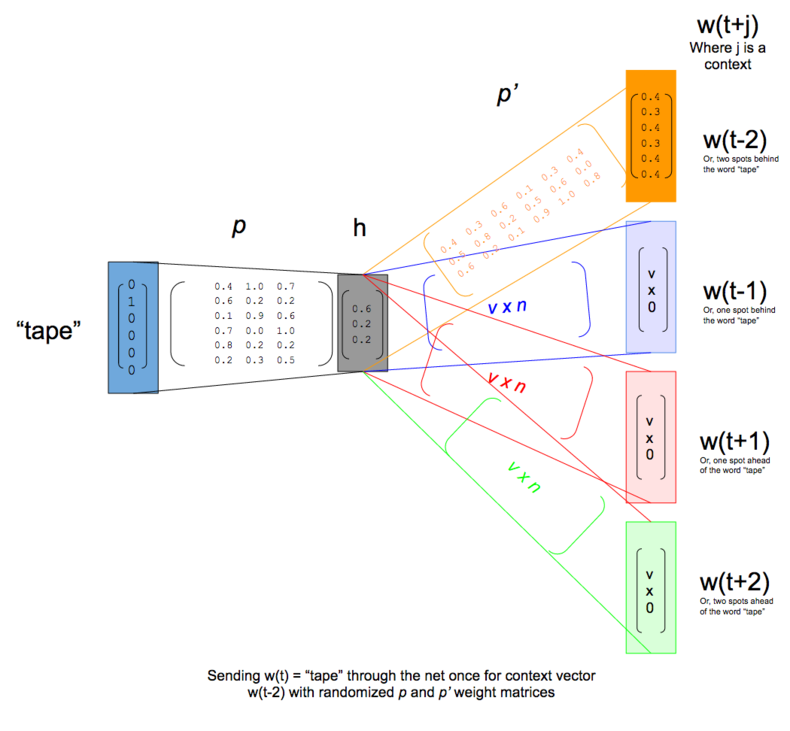
\includegraphics[scale=0.50]{./figures/skip-gram-exp.png}
  \end{frame}

  \begin{frame}{Word2Vec}
      La capa de input tiene tantas neuronas como palabras en el vocabulario. La función de activación es lineal.

      \centering
      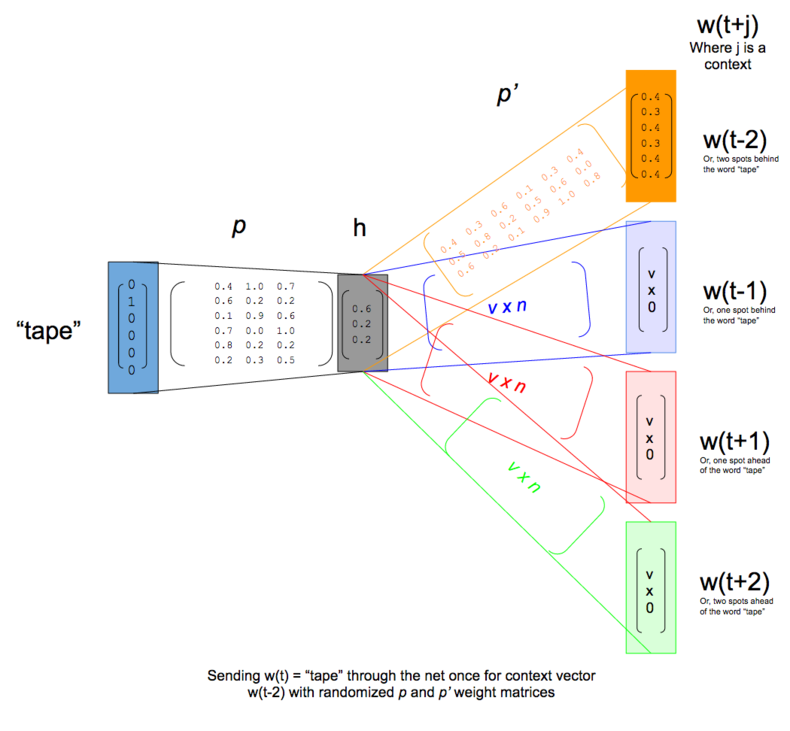
\includegraphics[scale=0.50]{./figures/skip-gram-exp.png}
  \end{frame}

  \begin{frame}{Word2Vec}
      h tiene tantas neuronas como componentes se quieran extraer.

      \centering
      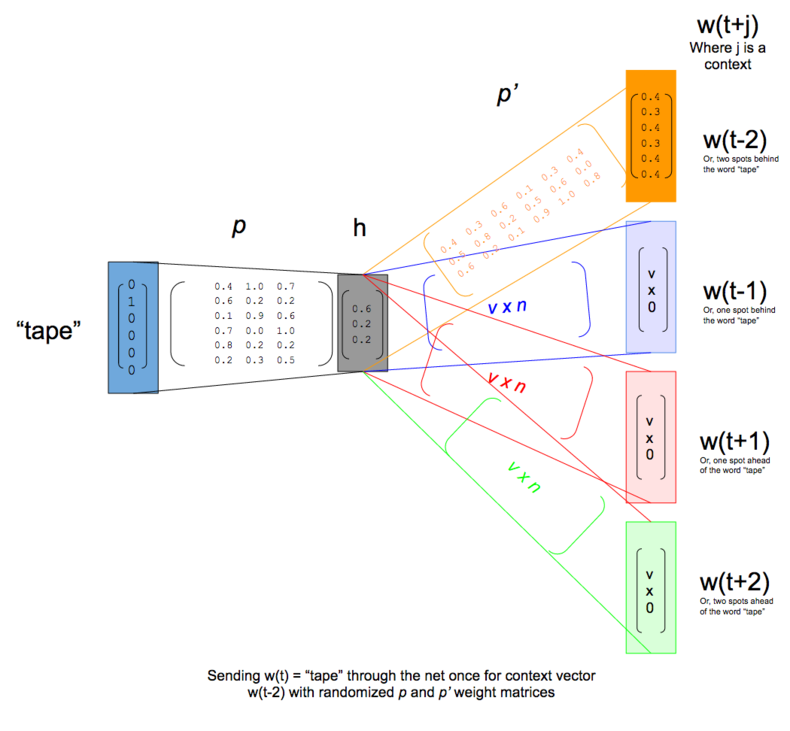
\includegraphics[scale=0.50]{./figures/skip-gram-exp.png}
  \end{frame}

  \begin{frame}{Word2Vec}
      La capa output tienen tantos vectores como el número de componentes de la ventana.

      \centering
      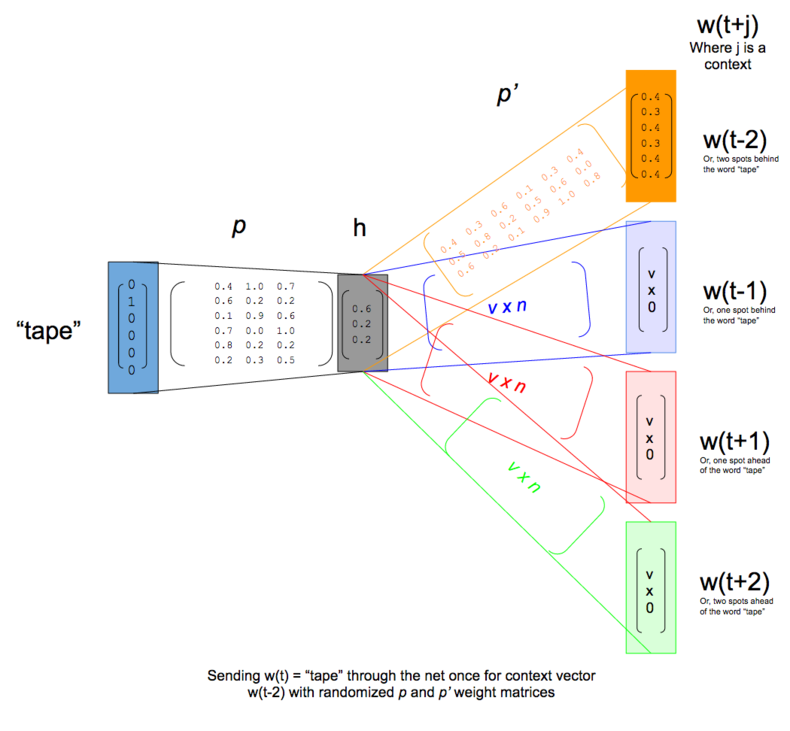
\includegraphics[scale=0.50]{./figures/skip-gram-exp.png}
  \end{frame}

  \begin{frame}{Word2Vec}
      Los resultados son vectores que se pueden comparar usando la similaridad del coseno de cada vector.

      \centering
      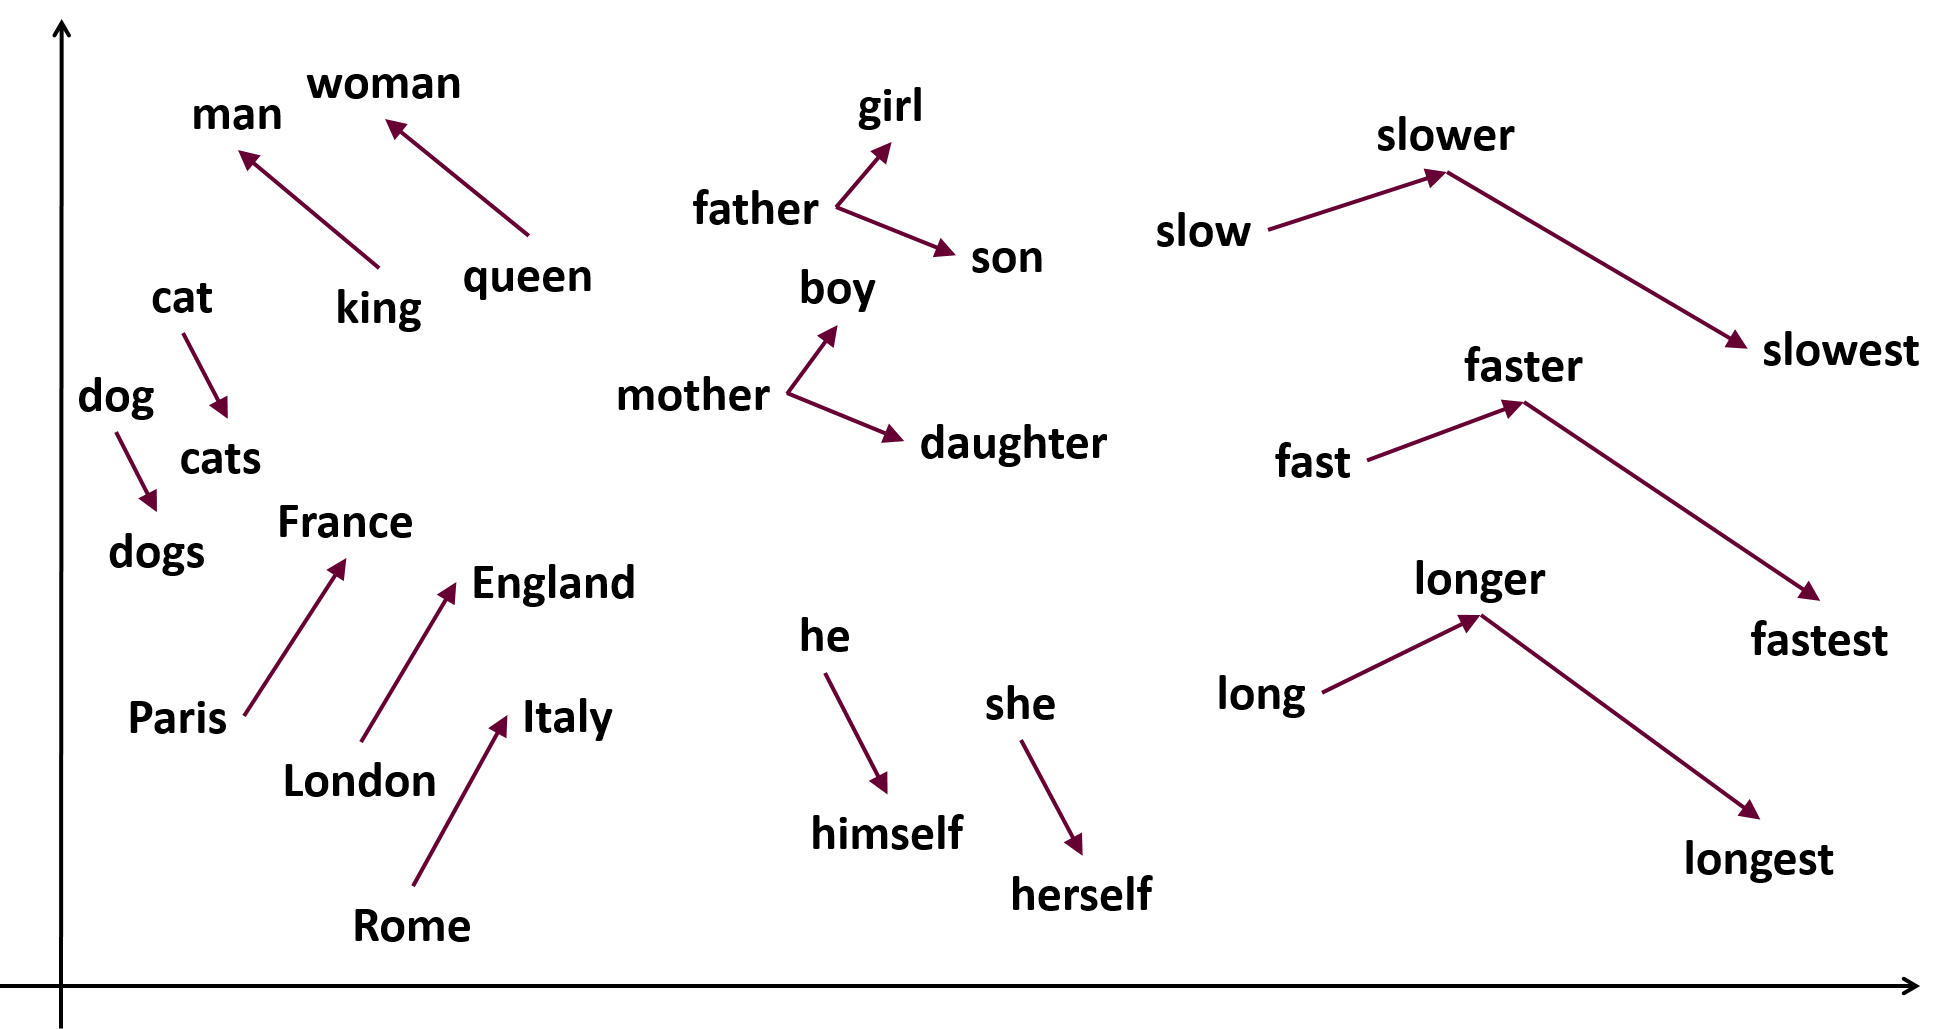
\includegraphics[width=\textwidth]{./figures/res-w2v.png}
  \end{frame}

  \begin{frame}{Word2Vec}
      \tiny
      \rowcolors{2}{gray!25}{white}
      \begin{table}
          \begin{tabularx}{\textwidth}{XXXXXX}
              \toprule
              \hiderowcolors Palabra clave & \multicolumn{5}{c}{Palabras similares}\\ \showrowcolors
              \midrule
              \textbf{mafia} & dealer & banker & mob & mexican & drug\\
              \textbf{axe} & expedition & undercover & biker & employee & outlaw\\
              \textbf{hair} & clothes & coat & eyes & teeth & makeup\\
              \textbf{airplane} & announcer & sanctuary & engine & accident & ambushed\\
              \textbf{plant} & retrieve & investigate & thwart & unearth & escape\\
              \textbf{air} & automatic & oil & swinging & oxygen & ocean\\
              \bottomrule
          \end{tabularx}
      \end{table}
  \end{frame}

  \begin{frame}{Doc2Vec}
      Word2Vec trabaja a nivel de palabras. Doc2Vec extiende el algoritmo para hacer comparaciones entre documentos.

      \centering
      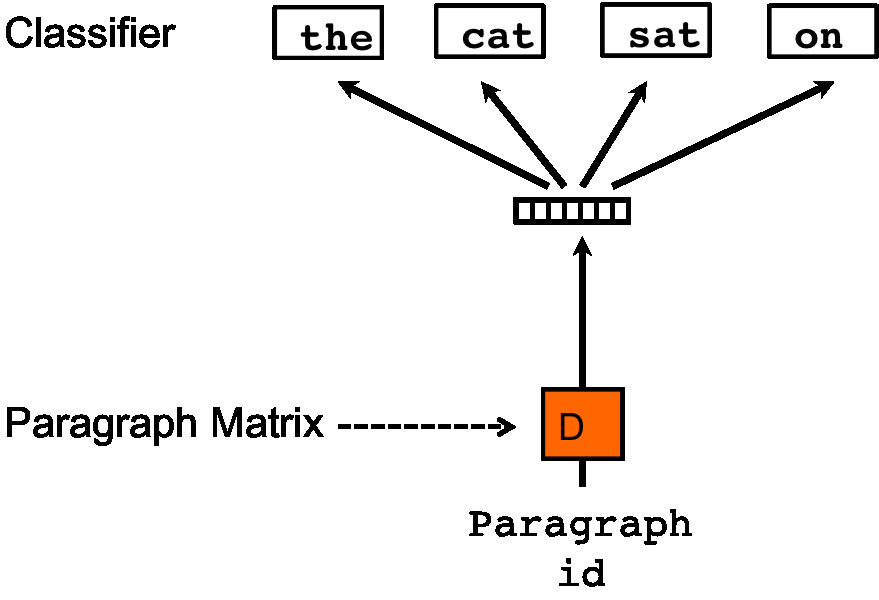
\includegraphics[scale=0.50]{./figures/distributed_bag_of_words.pdf}
  \end{frame}

  \section{E-Modelo}

  \begin{frame}{E-Modelo}
      Modelo de predicción de tokens hibrido.

      Combina el filtrado colaborativo con los features extraidos de un filtrado por contenido.
  \end{frame}

  \begin{frame}{E-Modelo}
      En primer lugar extraemos tokens como se ha hecho en el pre-filtrado de textos.

      En este caso se ha usado un servicio comercial llamado Bitext.
  \end{frame}

  \begin{frame}[fragile]{E-Modelo}
      \small
      \centering
      \begin{tikzpicture}[every node/.style={anchor=north east,fill=white,minimum width=1cm,minimum height=5mm}]
          \matrix (mA) [draw,matrix of math nodes]
          {
              1 & 1 & 0 \\
              0 & 1 & 0 \\
              -1 & -1 & -1 \\
          };

          \matrix (mB) [draw,matrix of math nodes] at ($(mA.south west)+(1.5,0.7)$)
          {
              -1 & -1 & -1 \\
              0 & 2 & 0 \\
              -1 & -1 & -1 \\
          };

          \matrix (mC) [draw,matrix of math nodes] at ($(mB.south west)+(1.5,0.7)$)
          {
              -1 & -1 & -1 \\
              0 & 1 & 0 \\
              0 & 0 & 2 \\
          };

          \node[above=10pt of mA-1-1, rotate=45, yshift=1mm, xshift=8mm] (top-1) {Palabra 1};
          \node[above=10pt of mA-1-2, rotate=45, yshift=1mm, xshift=8mm] (top-2) {Palabra 2};
          \node[above=10pt of mA-1-3, rotate=45, yshift=1mm, xshift=8mm] (top-3) {Palabra 3};

          \node[left=12pt of mC-1-1] (left-1) {Usuario 1};
          \node[left=12pt of mC-2-1] (left-2) {Usuario 2};
          \node[left=12pt of mC-3-1] (left-3) {Usuario 3};

          \node[right=12pt of mC-2-3, yshift=-3mm] (right-1) {Producto 3};
          \node[right=12pt of mB-2-3, yshift=-3mm] (right-2) {Producto 2};
          \node[right=12pt of mA-2-3, yshift=-3mm] (right-3) {Producto 1};

          \draw[dashed](mA.north east)--(mC.north east);
          \draw[dashed](mA.north west)--(mC.north west);
          \draw[dashed](mA.south east)--(mC.south east);
      \end{tikzpicture}
  \end{frame}

  \begin{frame}[fragile]{E-Modelo}
      \tiny
      \begin{tikzpicture}[baseline=-0.65ex,scale=0.8,decoration=brace]
          \matrix [matrix of math nodes,left delimiter=(,right delimiter=),row sep=0.5cm,column sep=0.5cm] (m) {
              1 & 1 & 0 & -1 & -1 & -1 & -1 & -1 & -1 \\
              0 & 1 & 0 & 0 & 2 & 0 & 0 & 1 & 0 \\
              -1 & -1 & -1 & -1 & -1 & -1 & 0 & 0 & 2 \\
          };
          \node[above=10pt of m-1-1, rotate=45, yshift=3mm, xshift=3mm] (top-1) {Palabra 1};
          \node[above=10pt of m-1-2, rotate=45, yshift=3mm, xshift=3mm] (top-2) {Palabra 2};
          \node[above=10pt of m-1-3, rotate=45, yshift=3mm, xshift=3mm] (top-3) {Palabra 3};
          \node[above=10pt of m-1-4, rotate=45, yshift=3mm, xshift=3mm] (top-4) {Palabra 1};
          \node[above=10pt of m-1-5, rotate=45, yshift=3mm, xshift=3mm] (top-5) {Palabra 2};
          \node[above=10pt of m-1-6, rotate=45, yshift=3mm, xshift=3mm] (top-6) {Palabra 3};
          \node[above=10pt of m-1-7, rotate=45, yshift=3mm, xshift=3mm] (top-7) {Palabra 1};
          \node[above=10pt of m-1-8, rotate=45, yshift=3mm, xshift=3mm] (top-8) {Palabra 2};
          \node[above=10pt of m-1-9, rotate=45, yshift=3mm, xshift=3mm] (top-9) {Palabra 3};

          \node[left=20pt of m-1-1] (left-1) {Usuario 1};
          \node[left=20pt of m-2-1] (left-2) {Usuario 2};
          \node[left=15pt of m-3-1] (left-3) {Usuario 3}; % why not aligned?

          \draw[decorate,transform canvas={yshift=2cm},thick] (m-1-1.north west) -- node[above=2pt] {Producto 1} (m-1-3.north east);
          \draw[decorate,transform canvas={yshift=2cm},thick] (m-1-4.north west) -- node[above=2pt] {Producto 2} (m-1-6.north east);
          \draw[decorate,transform canvas={yshift=2cm},thick] (m-1-7.north west) -- node[above=2pt] {Producto 3} (m-1-9.north east);
      \end{tikzpicture}
  \end{frame}

  \section{Optimización}

  \begin{frame}{Optimización}
      Para cada modelo hay unos parámetros que se pueden ajustar.
  \end{frame}

  \begin{frame}{Parámetros LSA}
      \begin{itemize}
          \item Número de `features' TF-IDF
          \item Número de componentes LSA
          \item Frecuencia Mínima de Documentos
          \item Frecuencia Máxima de Documentos
      \end{itemize}
  \end{frame}

  \begin{frame}{Parámetros Doc2Vec}
      \begin{itemize}
          \item Size
          \item Window
          \item Minimum Word Count
          \item Iteraciones
      \end{itemize}
  \end{frame}

  \begin{frame}{Optimización LSA}
      \tiny
      \centering
      % This file was created by matplotlib2tikz v0.6.11.
\begin{tikzpicture}

\definecolor{color0}{rgb}{0.483870967741935,1,0.483870967741936}

\begin{axis}[
xlabel={Películas},
ylabel={Posición de la recomendación},
xmin=-0.283491355170685, xmax=4.30364514661012,
ymin=0, ymax=193.708522727273,
width=\figurewidth,
height=\figureheight,
xtick={0,1,2,3,4},
xticklabels={Paths of.,Full Metal.,Saving.,Platoon,The Deer.},
tick align=outside,
xticklabel style = {rotate=45},
tick pos=left,
x grid style={lightgray!92.026143790849673!black},
y grid style={lightgray!92.026143790849673!black},
legend entries={{feat 2000 cmpn 1000 mndf 5 mxdf 100 keyw 0\% lsa 100\% tot 233},{feat 5000 cmpn 1000 mndf 5 mxdf 100 keyw 0\% lsa 100\% tot 35},{feat None cmpn 1000 mndf 5 mxdf 100 keyw 0\% lsa 100\% tot 37}},
legend style={at={(0.03,0.97)}, anchor=north west, draw=white!80.0!black},
legend cell align={left}
]
\addplot [only marks, draw=blue!50.0!black, fill=blue!50.0!black, colormap/viridis]
table{%
x                      y
-1.094770710767571e-02 +2.000000000000000e+00
+1.017468476072540e+00 +7.000000000000000e+00
+1.995186422591863e+00 +8.000000000000000e+00
+3.013100378141341e+00 +3.300000000000000e+01
+4.070945393596619e+00 +1.830000000000000e+02
};
\addplot [only marks, draw=color0, fill=color0, colormap/viridis]
table{%
x                      y
-4.750546374654548e-02 +2.000000000000000e+00
+9.887907166319483e-01 +1.000000000000000e+00
+1.986315358609423e+00 +1.100000000000000e+01
+2.952746135679334e+00 +0.000000000000000e+00
+4.021598538543233e+00 +2.100000000000000e+01
};
\addplot [only marks, draw=red!50.0!black, fill=red!50.0!black, colormap/viridis]
table{%
x                      y
-4.452508350133422e-02 +2.000000000000000e+00
+1.030268324831481e+00 +1.000000000000000e+00
+2.077366621053750e+00 +1.100000000000000e+01
+2.948765299131759e+00 +0.000000000000000e+00
+3.965898891581123e+00 +2.300000000000000e+01
};
\addplot [semithick, blue!50.0!black, opacity=0.5, forget plot]
table {%
0 -31
1 7.80000000000003
2 46.6
3 85.4
4 124.2
};
\addplot [semithick, color0, opacity=0.5, forget plot]
table {%
0 -0.399999999999998
1 3.3
2 7
3 10.7
4 14.4
};
\addplot [semithick, red!50.0!black, opacity=0.5, forget plot]
table {%
0 -0.8
1 3.3
2 7.4
3 11.5
4 15.6
};
\end{axis}

\end{tikzpicture}
  \end{frame}

  \begin{frame}{Optimización LSA}
      \tiny
      \centering
      % This file was created by matplotlib2tikz v0.6.11.
\begin{tikzpicture}

\definecolor{color0}{rgb}{0.483870967741935,1,0.483870967741936}

\begin{axis}[
xlabel={Películas},
ylabel={Posición de la recomendación},
xmin=-0.433685551148337, xmax=6.3448234626804,
ymin=0, ymax=58.081737012987,
width=\figurewidth,
height=\figureheight,
xtick={0,1,2,3,4,5,6},
xticklabels={Gravity,Solaris,Interstellar,Alien,The Martian,Planet of.,Distrito 9},
tick align=outside,
xticklabel style = {rotate=45},
tick pos=left,
x grid style={lightgray!92.026143790849673!black},
y grid style={lightgray!92.026143790849673!black},
legend entries={{feat 2000 cmpn 1000 mndf 5 mxdf 100 keyw 0\% lsa 100\% tot 137},{feat 5000 cmpn 1000 mndf 5 mxdf 100 keyw 0\% lsa 100\% tot 117},{feat None cmpn 1000 mndf 5 mxdf 100 keyw 0\% lsa 100\% tot 96}},
legend style={at={(0.03,0.97)}, anchor=north west, draw=white!80.0!black},
legend cell align={left}
]
\addplot [only marks, draw=blue!50.0!black, fill=blue!50.0!black, colormap/viridis]
table{%
x                      y
-5.420625617958866e-03 +1.000000000000000e+00
+1.086622088194287e+00 +5.000000000000000e+00
+1.995440067901144e+00 +7.000000000000000e+00
+3.078365322052515e+00 +1.300000000000000e+01
+4.043780263625694e+00 +1.400000000000000e+01
+4.946125615546470e+00 +4.200000000000000e+01
+5.977704951936783e+00 +5.500000000000000e+01
};
\addplot [only marks, draw=color0, fill=color0, colormap/viridis]
table{%
x                      y
-8.528152414794855e-02 +1.000000000000000e+00
+9.718706170388742e-01 +4.000000000000000e+00
+2.107066229334886e+00 +1.000000000000000e+01
+2.922658544319798e+00 +1.100000000000000e+01
+4.069389572958468e+00 +1.300000000000000e+01
+5.083171633766593e+00 +2.700000000000000e+01
+5.979475177772462e+00 +5.100000000000000e+01
};
\addplot [only marks, draw=red!50.0!black, fill=red!50.0!black, colormap/viridis]
table{%
x                      y
-4.725123114241665e-02 +1.000000000000000e+00
+9.359426374888414e-01 +4.000000000000000e+00
+2.052841684428433e+00 +9.000000000000000e+00
+3.055576540820828e+00 +1.000000000000000e+01
+3.924672303573277e+00 +1.300000000000000e+01
+5.152248526925555e+00 +2.100000000000000e+01
+5.995823104116642e+00 +3.800000000000000e+01
};
\addplot [semithick, blue!50.0!black, opacity=0.5, forget plot]
table {%
0 -6.46428571428571
1 2.21428571428572
2 10.8928571428572
3 19.5714285714286
4 28.25
5 36.9285714285714
6 45.6071428571429
};
\addplot [semithick, color0, opacity=0.5, forget plot]
table {%
0 -4.60714285714285
1 2.50000000000001
2 9.60714285714286
3 16.7142857142857
4 23.8214285714286
5 30.9285714285714
6 38.0357142857143
};
\addplot [semithick, red!50.0!black, opacity=0.5, forget plot]
table {%
0 -2.25
1 3.07142857142857
2 8.39285714285714
3 13.7142857142857
4 19.0357142857143
5 24.3571428571429
6 29.6785714285714
};
\end{axis}

\end{tikzpicture}
  \end{frame}

  \begin{frame}{Optimización LSA}
      \tiny
      \centering
      % This file was created by matplotlib2tikz v0.6.11.
\begin{tikzpicture}

\definecolor{color0}{rgb}{0.483870967741935,1,0.483870967741936}

\begin{axis}[
xlabel={Películas},
ylabel={Posición de la recomendación},
xmin=-0.346640451275573, xmax=5.33750705174778,
ymin=0, ymax=346.329951298701,
width=\figurewidth,
height=\figureheight,
xtick={0,1,2,3,4,5},
xticklabels={Shrek,Monsters\, Inc.,Ponyo,The Incredibles,Toy Story 2,Totoro},
tick align=outside,
xticklabel style = {rotate=45},
tick pos=left,
x grid style={lightgray!92.026143790849673!black},
y grid style={lightgray!92.026143790849673!black},
legend style={at={(0.03,0.97)}, anchor=north west, draw=white!80.0!black},
legend entries={{feat 2000 cmpn 1000 mndf 5 mxdf 100 keyw 0\% lsa 100\% tot 578},{feat 5000 cmpn 1000 mndf 5 mxdf 100 keyw 0\% lsa 100\% tot 463},{feat None cmpn 1000 mndf 5 mxdf 100 keyw 0\% lsa 100\% tot 504}},
legend cell align={left}
]
\addplot [only marks, draw=blue!50.0!black, fill=blue!50.0!black, colormap/viridis]
table{%
x                      y
-5.802817474518601e-02 +1.000000000000000e+00
+9.438194535137451e-01 +7.000000000000000e+00
+1.917711120773622e+00 +1.000000000000000e+01
+3.006034283472499e+00 +2.400000000000000e+01
+4.031893351252491e+00 +3.270000000000000e+02
+4.934052430070538e+00 +2.090000000000000e+02
};
\addplot [only marks, draw=color0, fill=color0, colormap/viridis]
table{%
x                      y
+6.366498802012376e-02 +2.000000000000000e+00
+9.992390653301425e-01 +7.000000000000000e+00
+2.010737632320609e+00 +1.300000000000000e+01
+2.970734959804123e+00 +1.700000000000000e+01
+4.003118802453389e+00 +1.710000000000000e+02
+5.027275653882869e+00 +2.530000000000000e+02
};
\addplot [only marks, draw=red!50.0!black, fill=red!50.0!black, colormap/viridis]
table{%
x                      y
+6.635168283415073e-02 +2.000000000000000e+00
+9.788464956280608e-01 +5.000000000000000e+00
+1.987999875649677e+00 +1.400000000000000e+01
+2.888126863936821e+00 +1.300000000000000e+01
+3.945887347519687e+00 +1.580000000000000e+02
+5.044876595228294e+00 +3.120000000000000e+02
};
\addplot [semithick, blue!50.0!black, opacity=0.5, forget plot]
table {%
0 -47.5238095238095
1 10.0190476190476
2 67.5619047619047
3 125.104761904762
4 182.647619047619
5 240.190476190476
};
\addplot [semithick, color0, opacity=0.5, forget plot]
table {%
0 -47.9047619047619
1 2.12380952380954
2 52.152380952381
3 102.180952380952
4 152.209523809524
5 202.238095238095
};
\addplot [semithick, red!50.0!black, opacity=0.5, forget plot]
table {%
0 -59.4285714285714
1 -2.05714285714287
2 55.3142857142857
3 112.685714285714
4 170.057142857143
5 227.428571428571
};
\end{axis}

\end{tikzpicture}

  \end{frame}

  \begin{frame}{Optimización Doc2Vec}
      \tiny
      \centering
      % This file was created by matplotlib2tikz v0.6.11.
\begin{tikzpicture}

\definecolor{color0}{rgb}{0,0.833333333333333,1}
\definecolor{color1}{rgb}{1,0.901234567901234,0}

\begin{axis}[
xlabel={Películas},
ylabel={Posición de la recomendación},
xmin=-0.318878784803842, xmax=4.29478961344254,
ymin=0, ymax=15.8744761320024,
width=\figurewidth,
height=\figureheight,
xtick={0,1,2,3,4},
xticklabels={Saving Private.,The Deer Hunter,Platoon,Full Metal.,Paths of Glory},
tick align=outside,
xticklabel style = {rotate=45},
tick pos=left,
x grid style={lightgray!92.026143790849673!black},
y grid style={lightgray!92.026143790849673!black},
legend style={at={(0.03,0.97)}, anchor=north west, draw=white!80.0!black},
legend cell align={left},
legend entries={{size 1000 window 5 minc 5 iter 5 tot 26},{size 1000 window 5 minc 5 iter 10 tot 20},{size 1000 window 5 minc 5 iter 20 tot 23},{size 1000 window 5 minc 5 iter 30 tot 26}}
]
\addplot [only marks, draw=blue!50.0!black, fill=blue!50.0!black, colormap/viridis]
table{%
x                      y
-4.785763806766297e-02 +2.000000000000000e+00
+9.627603052816800e-01 +6.000000000000000e+00
+1.955623678099405e+00 +9.000000000000000e+00
+2.996166223203151e+00 +4.000000000000000e+00
+3.958191491405981e+00 +5.000000000000000e+00
};
\addplot [only marks, draw=color0, fill=color0, colormap/viridis]
table{%
x                      y
+6.749129676971040e-02 +2.000000000000000e+00
+9.979280597101551e-01 +1.000000000000000e+00
+2.005808910197287e+00 +8.000000000000000e+00
+3.027450171149013e+00 +3.000000000000000e+00
+4.037931308297460e+00 +6.000000000000000e+00
};
\addplot [only marks, draw=color1, fill=color1, colormap/viridis]
table{%
x                      y
-8.164169225530499e-02 +3.000000000000000e+00
+9.950779869551548e-01 +2.000000000000000e+00
+1.954352266828085e+00 +0.000000000000000e+00
+3.075912459844018e+00 +7.000000000000000e+00
+4.057552520894004e+00 +1.100000000000000e+01
};
\addplot [only marks, draw=red!50.0!black, fill=red!50.0!black, colormap/viridis]
table{%
x                      y
-3.780992218467522e-02 +3.000000000000000e+00
+1.044659612228541e+00 +2.000000000000000e+00
+2.005356539524874e+00 +0.000000000000000e+00
+2.988538031311266e+00 +6.000000000000000e+00
+3.962289868063661e+00 +1.500000000000000e+01
};
\addplot [semithick, blue!50.0!black, opacity=0.5, forget plot]
table {%
0 4.4
1 4.8
2 5.2
3 5.6
4 6
};
\addplot [semithick, color0, opacity=0.5, forget plot]
table {%
0 2
1 3
2 4
3 5
4 6
};
\addplot [semithick, color1, opacity=0.5, forget plot]
table {%
0 0.400000000000001
1 2.5
2 4.6
3 6.7
4 8.8
};
\addplot [semithick, red!50.0!black, opacity=0.5, forget plot]
table {%
0 -0.399999999999998
1 2.4
2 5.2
3 8.00000000000001
4 10.8
};
\end{axis}

\end{tikzpicture}
  \end{frame}

  \begin{frame}{Optimización Doc2Vec}
      \tiny
      \centering
      % This file was created by matplotlib2tikz v0.6.11.
\begin{tikzpicture}

\definecolor{color0}{rgb}{0,0.833333333333333,1}
\definecolor{color1}{rgb}{1,0.901234567901234,0}

\begin{axis}[
xlabel={Películas},
ylabel={Posición de la recomendación},
xmin=-0.337159373980144, xmax=6.36547218879069,
ymin=0, ymax=121.103165584416,
width=\figurewidth,
height=\figureheight,
xtick={0,1,2,3,4,5,6},
xticklabels={Solaris,Interstellar,Planet of the.,Alien,Distrito 9,Gravity,The Martian},
tick align=outside,
xticklabel style = {rotate=45},
tick pos=left,
x grid style={lightgray!92.026143790849673!black},
y grid style={lightgray!92.026143790849673!black},
legend style={at={(0.03,0.97)}, anchor=north west, draw=white!80.0!black},
legend entries={{size 1000 window 5 minc 5 iter 5 tot 222},{size 1000 window 5 minc 5 iter 10 tot 161},{size 1000 window 5 minc 5 iter 20 tot 96},{size 1000 window 5 minc 5 iter 30 tot 116}},
legend cell align={left}
]
\addplot [only marks, draw=blue!50.0!black, fill=blue!50.0!black, colormap/viridis]
table{%
x                      y
+7.623543280607674e-03 +0.000000000000000e+00
+9.444215350133989e-01 +2.000000000000000e+01
+1.964080953665051e+00 +2.400000000000000e+01
+2.967717353347173e+00 +3.200000000000000e+01
+4.040133610939218e+00 +3.000000000000000e+00
+4.867595562679769e+00 +2.800000000000000e+01
+6.006787316057554e+00 +1.150000000000000e+02
};
\addplot [only marks, draw=color0, fill=color0, colormap/viridis]
table{%
x                      y
+7.902383706499691e-03 +0.000000000000000e+00
+1.033795190538360e+00 +8.000000000000000e+00
+1.961077227382269e+00 +1.600000000000000e+01
+2.942263835717434e+00 +1.400000000000000e+01
+3.938882033585026e+00 +1.500000000000000e+01
+4.997316046512450e+00 +3.400000000000000e+01
+6.006871894193711e+00 +7.400000000000000e+01
};
\addplot [only marks, draw=color1, fill=color1, colormap/viridis]
table{%
x                      y
+4.837745136153115e-02 +0.000000000000000e+00
+1.152033758409714e+00 +3.000000000000000e+00
+2.063846874851872e+00 +4.000000000000000e+00
+2.967907485967270e+00 +9.000000000000000e+00
+4.002867362698304e+00 +2.300000000000000e+01
+5.059388781421315e+00 +1.400000000000000e+01
+5.970813400844059e+00 +4.300000000000000e+01
};
\addplot [only marks, draw=red!50.0!black, fill=red!50.0!black, colormap/viridis]
table{%
x                      y
+7.778597005651774e-02 +0.000000000000000e+00
+9.723276855200051e-01 +1.000000000000000e+00
+1.993960965661173e+00 +5.000000000000000e+00
+3.052109105123921e+00 +8.000000000000000e+00
+4.008150870553743e+00 +3.200000000000000e+01
+4.886701888253074e+00 +1.600000000000000e+01
+6.020357082440115e+00 +5.400000000000000e+01
};
\addplot [semithick, blue!50.0!black, opacity=0.5, forget plot]
table {%
0 -4.7142857142857
1 7.42857142857144
2 19.5714285714286
3 31.7142857142857
4 43.8571428571429
5 56
6 68.1428571428572
};
\addplot [semithick, color0, opacity=0.5, forget plot]
table {%
0 -6.24999999999999
1 3.50000000000001
2 13.25
3 23
4 32.75
5 42.5
6 52.25
};
\addplot [semithick, color1, opacity=0.5, forget plot]
table {%
0 -4.49999999999999
1 1.57142857142858
2 7.64285714285715
3 13.7142857142857
4 19.7857142857143
5 25.8571428571429
6 31.9285714285714
};
\addplot [semithick, red!50.0!black, opacity=0.5, forget plot]
table {%
0 -6.89285714285713
1 0.928571428571439
2 8.75000000000001
3 16.5714285714286
4 24.3928571428571
5 32.2142857142857
6 40.0357142857143
};
\end{axis}

\end{tikzpicture}
  \end{frame}

  \begin{frame}{Optimización Doc2Vec}
      \tiny
      \centering
      % This file was created by matplotlib2tikz v0.6.11.
\begin{tikzpicture}

\definecolor{color0}{rgb}{0,0.833333333333333,1}
\definecolor{color1}{rgb}{1,0.901234567901234,0}

\begin{axis}[
xlabel={Películas},
ylabel={Posición de la recomendación},
xmin=-0.312341057262753, xmax=5.33409239877808,
ymin=0, ymax=87.8857142857143,
width=\figurewidth,
height=\figureheight,
xtick={0,1,2,3,4,5},
xticklabels={The Incredibles,Ponyo,Totoro,Monsters\, Inc.,Toy Story 2,Shrek},
tick align=outside,
xticklabel style = {rotate=45},
tick pos=left,
x grid style={lightgray!92.026143790849673!black},
y grid style={lightgray!92.026143790849673!black},
legend style={at={(0.03,0.97)}, anchor=north west, draw=white!80.0!black},
legend cell align={left},
legend entries={{size 1000 window 5 minc 5 iter 5 tot 243},{size 1000 window 5 minc 5 iter 10 tot 126},{size 1000 window 5 minc 5 iter 20 tot 114},{size 1000 window 5 minc 5 iter 30 tot 105}}
]
\addplot [only marks, draw=blue!50.0!black, fill=blue!50.0!black, colormap/viridis]
table{%
x                      y
+2.854210361233427e-02 +3.000000000000000e+00
+9.985860941212598e-01 +1.700000000000000e+01
+1.989719734384425e+00 +1.200000000000000e+01
+2.977518934895279e+00 +5.200000000000000e+01
+4.047838581534850e+00 +8.300000000000000e+01
+5.047194397110533e+00 +7.600000000000000e+01
};
\addplot [only marks, draw=color0, fill=color0, colormap/viridis]
table{%
x                      y
+5.047449785200740e-02 +1.000000000000000e+00
+1.006637893034865e+00 +4.000000000000000e+00
+1.992916348248827e+00 +1.000000000000000e+01
+2.975148908453217e+00 +3.100000000000000e+01
+4.062908908683289e+00 +3.600000000000000e+01
+4.989111717822619e+00 +4.400000000000000e+01
};
\addplot [only marks, draw=color1, fill=color1, colormap/viridis]
table{%
x                      y
-2.189235127517257e-02 +0.000000000000000e+00
+1.065277596823530e+00 +6.000000000000000e+00
+2.035357183128240e+00 +2.200000000000000e+01
+3.087593759253258e+00 +2.100000000000000e+01
+3.915765071576033e+00 +3.000000000000000e+01
+5.015058767498841e+00 +3.500000000000000e+01
};
\addplot [only marks, draw=red!50.0!black, fill=red!50.0!black, colormap/viridis]
table{%
x                      y
+6.722550225743713e-03 +0.000000000000000e+00
+9.246839503806149e-01 +4.000000000000000e+00
+2.041799048071679e+00 +1.900000000000000e+01
+2.972694804836483e+00 +1.200000000000000e+01
+4.071179803783091e+00 +2.900000000000000e+01
+5.009386032868991e+00 +4.100000000000000e+01
};
\addplot [semithick, blue!50.0!black, opacity=0.5, forget plot]
table {%
0 -2.57142857142858
1 14.6571428571428
2 31.8857142857143
3 49.1142857142857
4 66.3428571428571
5 83.5714285714286
};
\addplot [semithick, color0, opacity=0.5, forget plot]
table {%
0 -2.71428571428572
1 6.77142857142857
2 16.2571428571428
3 25.7428571428571
4 35.2285714285714
5 44.7142857142857
};
\addplot [semithick, color1, opacity=0.5, forget plot]
table {%
0 1.42857142857143
1 8.45714285714285
2 15.4857142857143
3 22.5142857142857
4 29.5428571428571
5 36.5714285714286
};
\addplot [semithick, red!50.0!black, opacity=0.5, forget plot]
table {%
0 -2
1 5.79999999999999
2 13.6
3 21.4
4 29.2
5 37
};
\end{axis}

\end{tikzpicture}

  \end{frame}

  \section{Demo}

  \begin{frame}{Demo}
      \url{https://moviepepper.hugofs.com}
  \end{frame}
\end{document}
